\section{Koncept \& Prototype}

Dataman, se figur \ref{fig:Dataman} er en databank man har på sin person når man ønsker at indsamle alt data omkring ens færden, fysiske aktivitet og omgivelser. Dataman indsamler GPS koordinater, puls, temperaturer, lys niveauer, og optager alt lyd. Man kan på sin Dataman slukke og tænde manuelt for optagelse af data ved en on/off switch som viser sig som en oplys rød LED for at man ikke optager, og en grøn LED for at man optager. 
Man kan igennem et specielt håndtryk, udveksle data med hinanden. 
Alt data bliver visualiseret og styret igennem et interface på ens mobile enhed, eller computer, i form af en graf og en liste af rå data. Man kan slette data fra sin historik som man vil, men dette fremgår så som et hul i sin data historik. 
Man kan også sælge sin data. Det opbygger en vis værdi, som fluktuerer baseret på ens omgivelser og hvad man laver. F.eks. er dataen mere værd i centrum i en by omgivet af andre mennesker. Dataen for en pågældende dag bliver solgt hvis man vælger dette, man kan dog også vælge at donere sine data til et velgørende formål. 


\subsection{Prototype}
Dataman prototypen\ref{fig:Dataman} består af en Sparkcore enhed der indsamler data fra en temperatursensor, en puls sensor der sidder på spidsen af en finger, en lyssensor der måler lysniveauet, en lyd sensor der måler det generelle lyd tryk i ens omgivelser, og GPS koordinaterne fra ens tilkoblet enhed. Disse data sendes igennem wifi op til en cloudløsning fra producenten af sparkcore med HTTP igennem en API. Disse data tilgåes igennem samme API og bruges Javascript frameworket ReactJS. React formidler dataen op til HTML elementer som man så kan se live på en graf i ens browser, se figur \ref{fig:ui}. Dataen ses også som en løbende tabel under grafen. Data her kan slettes som man lyster.

\begin{figure}
    \centering
    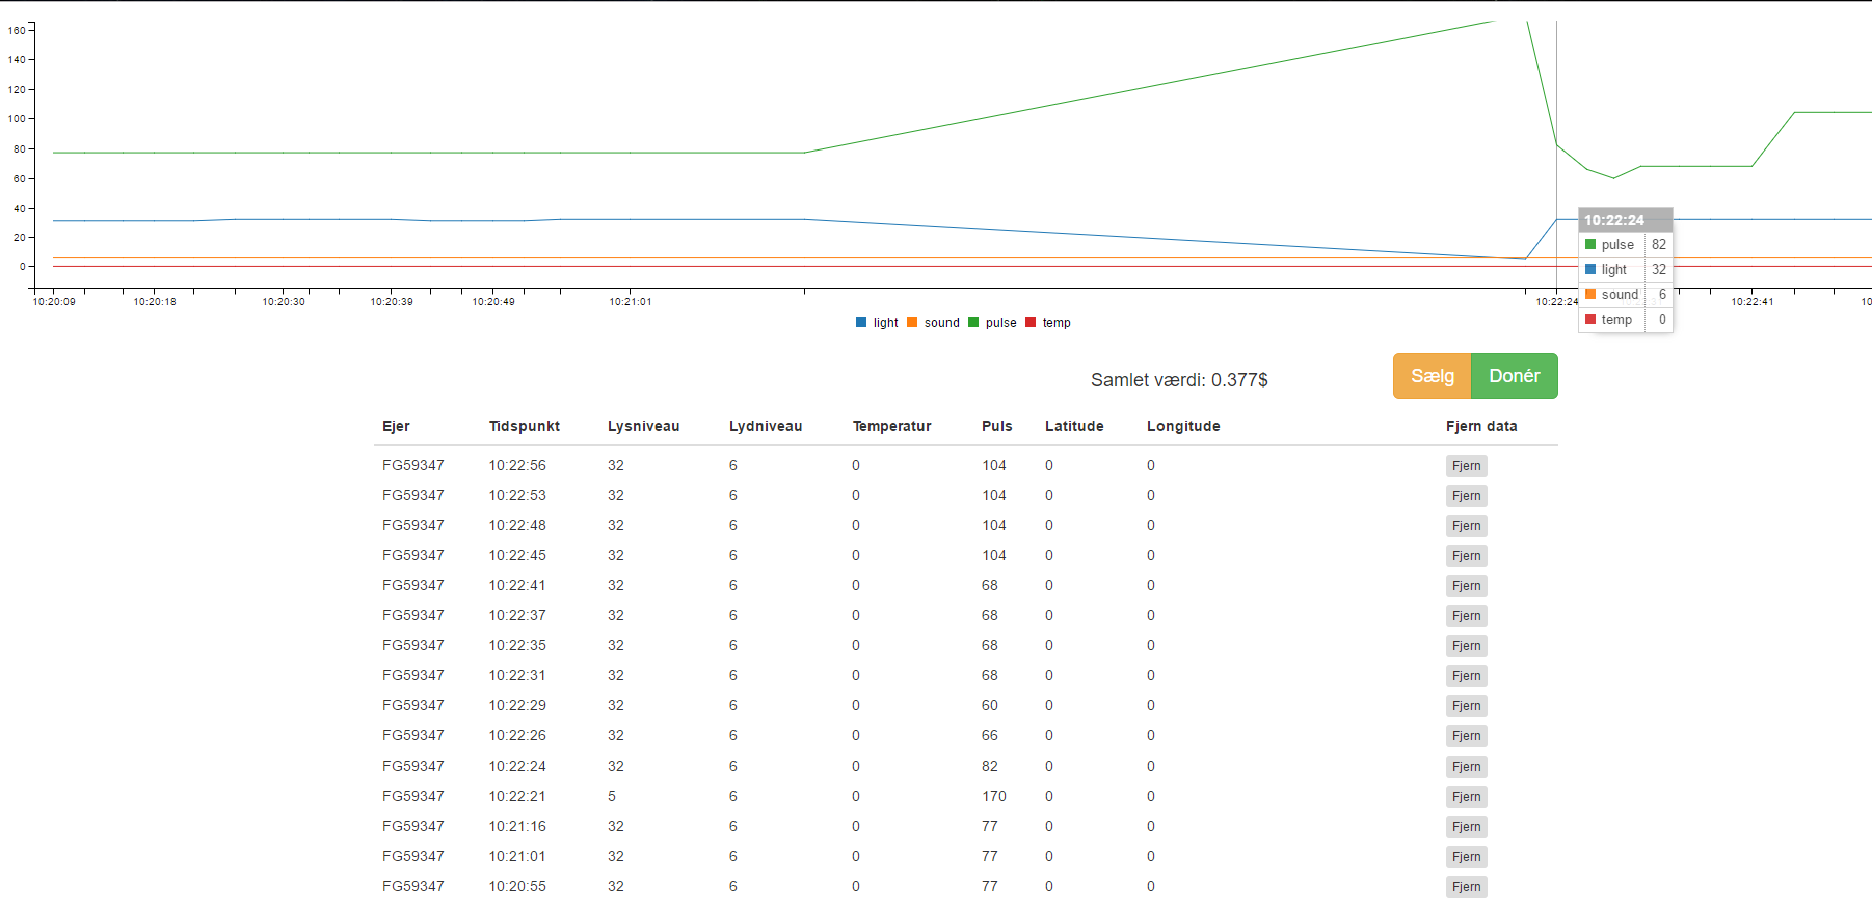
\includegraphics[width = \textwidth]{Pictures/datamanui.png}
    \caption{Datamans UI}
    \label{fig:ui}
\end{figure}

\begin{figure}
    \centering
    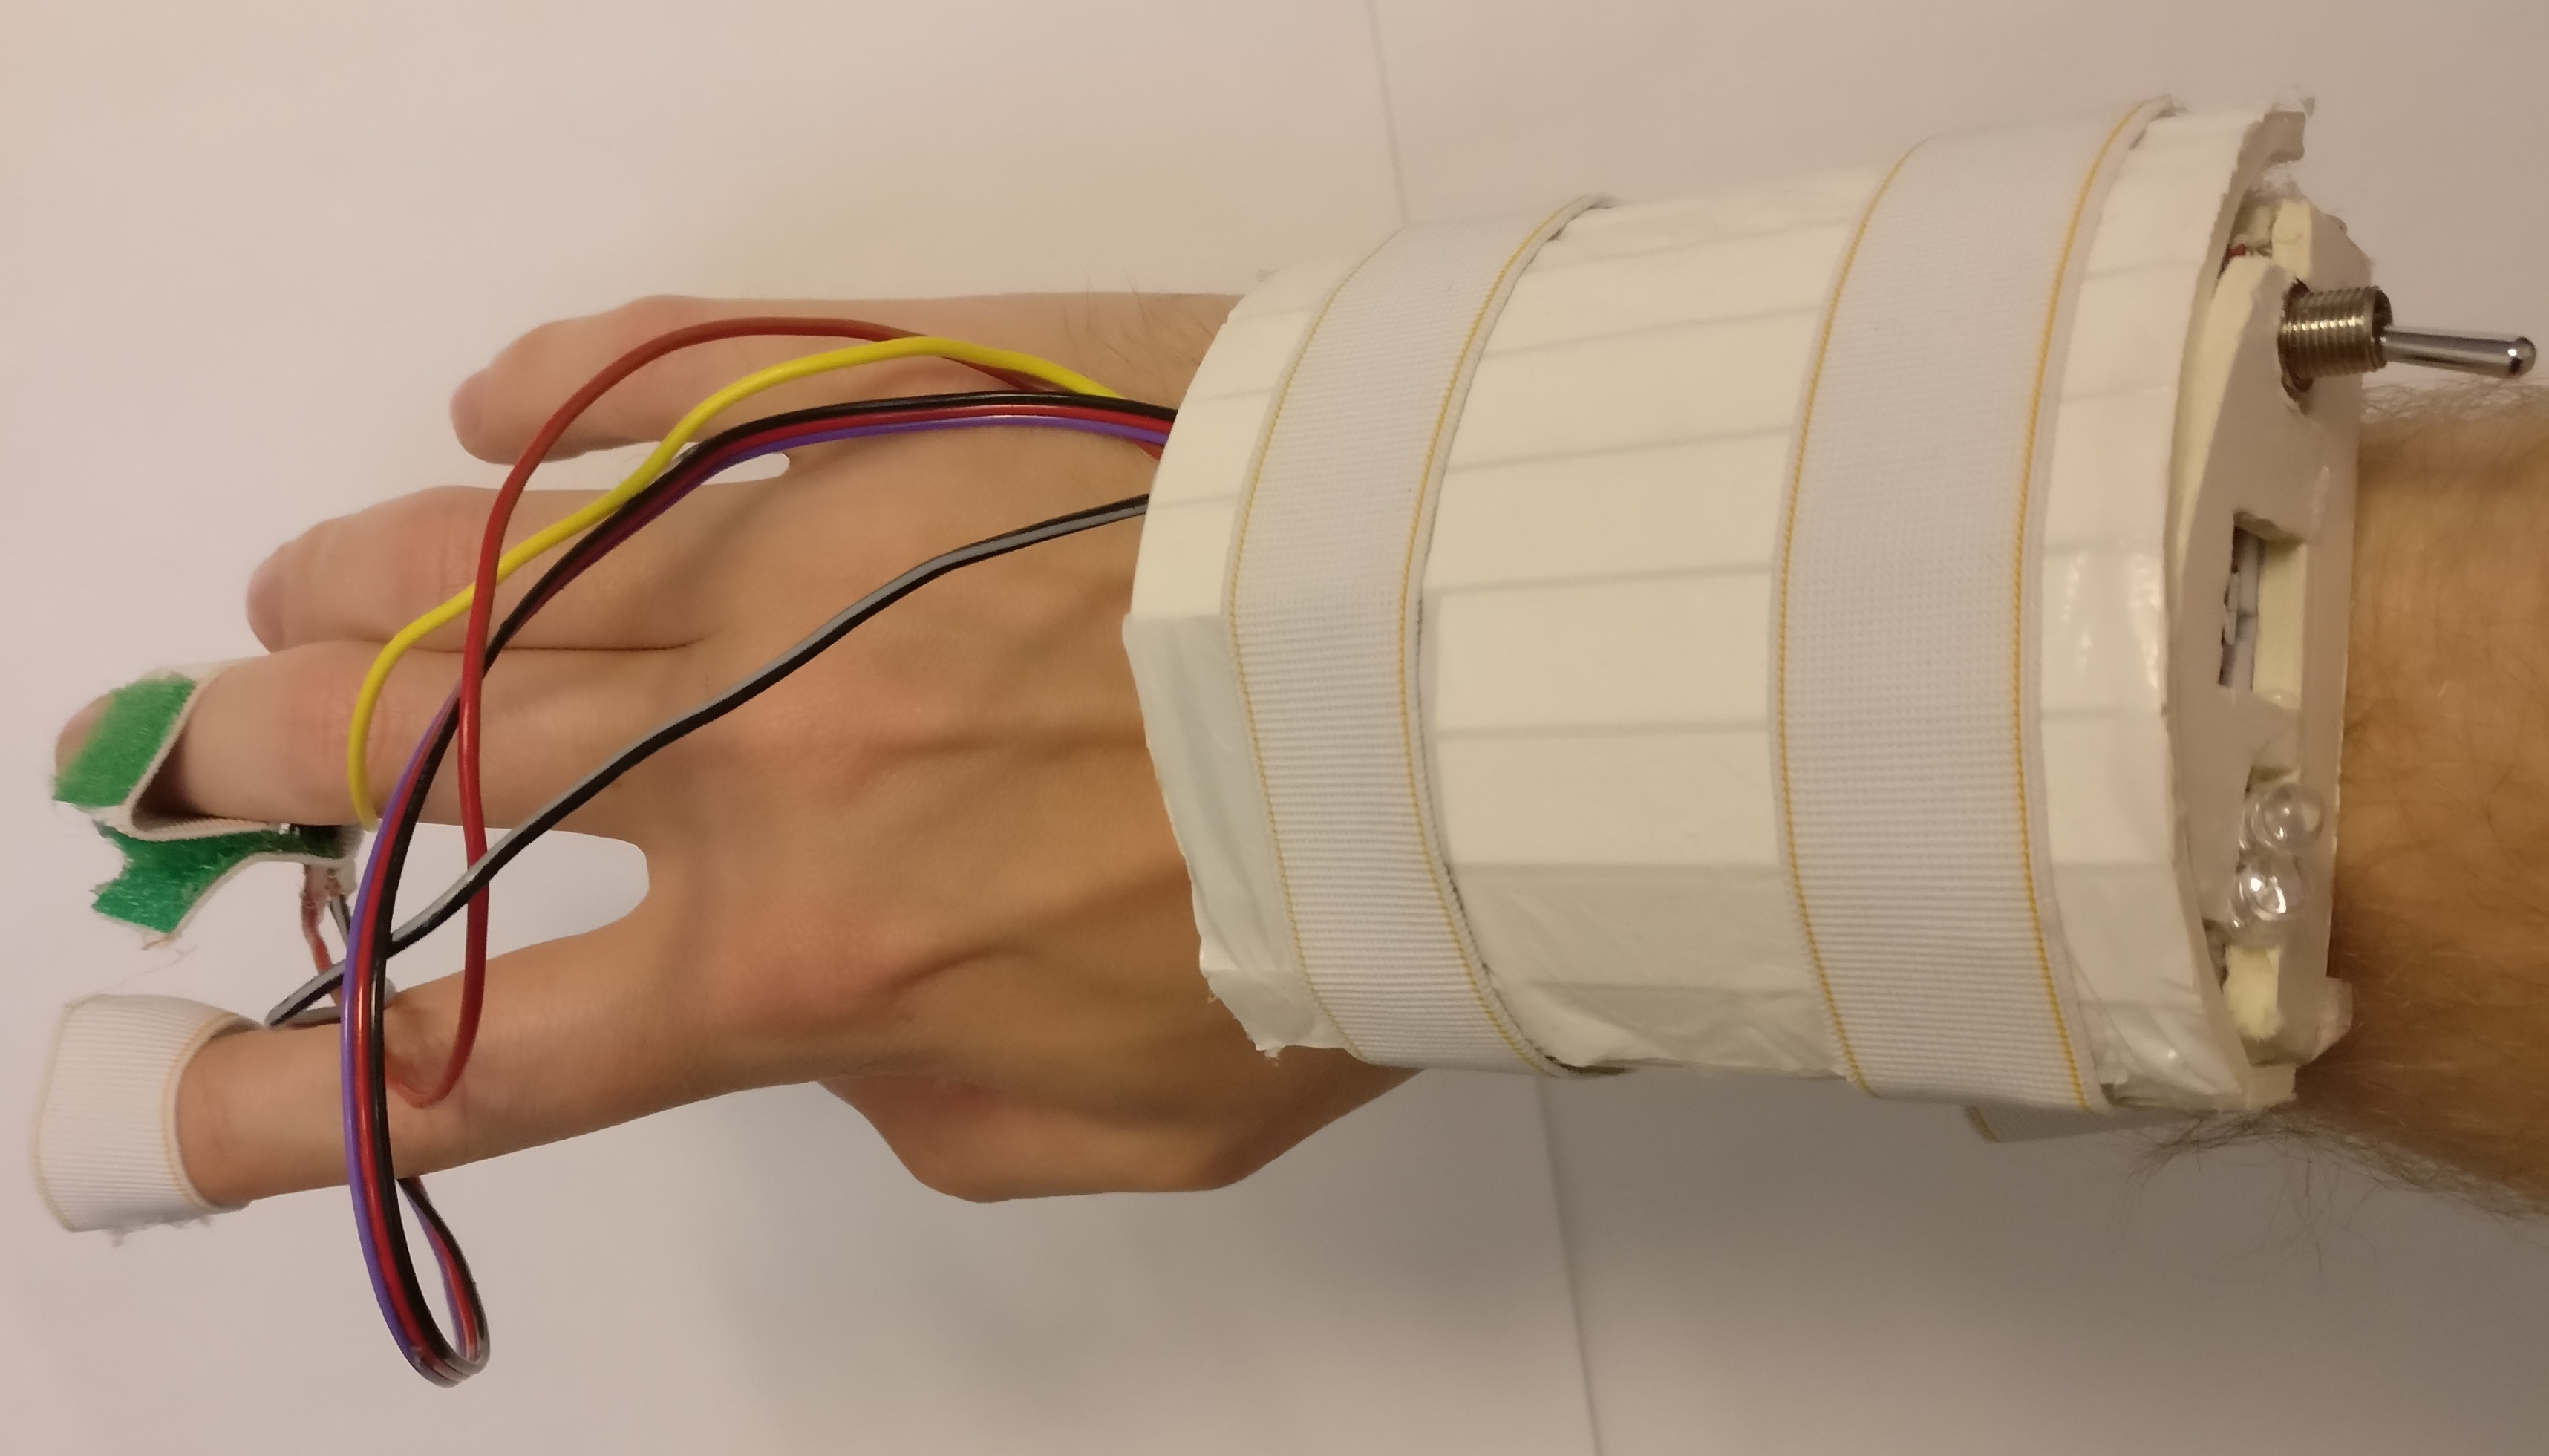
\includegraphics[width = \textwidth]{Pictures/Dataman.jpg}
    \caption{Dataman prototype}
    \label{fig:Dataman}
\end{figure}


\begin{comment}

HUSK AT SKRIVE OM WEBINTERFACE

\end{comment}
